\chapter{Marco teórico: Autómatas celulares}

Un autómata celular, concebido por John von Neumann \cite{vonNeumann1948}, es una colección de células que pueden adquirir un estado y que se agrupan en una red. El autómata celular evoluciona en pasos de tiempo, donde cada célula cambia su estado en función de los estados de su vecindad.  Además, durante la evolución cambia de una configuración a otra \cite{weissteinCA, wolfram1982, ca_fsancho}. 

Tradicionalmente, se considera una red regular de células, un conjunto finito de estados y evoluciones en pasos discretos de tiempo.

\begin{definition}
	
	Un autómata celular es una 4-tupla ($\mathcal{L}, \mathcal{S}, \mathcal{N}, \mathcal{R}$) donde:
	
	
	
	\begin{itemize}
		
		\item $\mathcal{L} \subseteq \mathbb{Z}^D$ es el espacio celular $D$-dimensional. Un conjunto de células se coloca en el espacio $\mathcal{L}$ para formar una red.
		
		
		
		\item $\mathcal{S}$ es un conjunto de estados. Cada célula solo puede adquirir un valor de un conjunto finito de diferentes valores:
		
		\[
		\sigma_{\vec{i}}(t) \in \mathcal{S} \equiv \{ 0, 1,2, \dots, k - 1 \},\; \forall \vec{i} \in \mathcal{L}
		\]
		
		Donde $\vec{i} \in \mathcal{L}$ es una célula en el espacio celular, $\sigma_{\vec{i}} (t)$ es el estado de la i-ésima célula en el tiempo $t$ y $\mathcal{S}$ es un anillo conmutativo finito\footnote{Un anillo conmutativo finito es un conjunto con suma y multiplicación, donde la suma se comporta como una suma normal (conmutativa e inversa), la multiplicación también es conmutativa y ambas operaciones cumplen la propiedad distributiva.}, generalmente definido por los enteros módulo $k$ ($\mathbb{Z}_k$).
		
		
		
		\item $\mathcal{N} = (\vec{v}_1, \vec{v}_2, \dots, \vec{v}_m )$ es el conjunto de vectores de desplazamiento que definen la vecindad de una célula en $\mathcal{L}$. Así, los vecinos de las células ubicadas en $\vec{i} \in \mathcal{L}$ se encuentran en las posiciones $\vec{i} + \vec{v}_j, \forall j \in \{ 1,2, \dots, m \}$ 
		
		
		
		\item $\mathcal{R} : \mathcal{S}^m \to \mathcal{S}$ es la regla local del autómata:
		
		\[
		\sigma_{\vec{i}}(t + 1) = \mathcal{R} ( \{ \sigma_{\vec{i} + \vec{v}_j}\}_{j = 1}^m  )
		\]
		
		donde $\mathcal{R}$ es la función de transición local que asigna el nuevo estado de una célula a partir de los estados de sus $m$ vecinos.
		
		
		
	\end{itemize}
	
\end{definition}

Esta formulación sigue de manera general a \cite{ca_phd, sayama_cellularautomata, ca_discrete_universe}.

\section{Vecindad}

La vecindad de una célula está estrechamente relacionada con la dimensionalidad del autómata celular. John von Neumann propone una vecindad para $\mathbb{Z}^2$ de cinco células formada por ella misma y las cuatro células ortogonales más cercanas \cite{ca_theory_self_reproduction} como se observa en la figura \ref{fig:N_neumann}. Esta vecindad es expandida por Moore añadiendo los cuatro vecinos diagonales más cercanos, dando una vecindad de nueve elementos \cite{moore}. Esta vecindad, representada por la figura \ref{fig:N_moore}, fue utilizada por John Conway en el ``Juego de la Vida'' \cite{life}.

La figura \ref{fig:N_wolfram} representa una vecindad de radio uno en un espacio unidimensional, es decir, todas aquellas células a una distancia menor o igual a uno, incluyéndose a su misma. Fue utilizada por Stephen Wolfram para definir los Autómatas Celulares Elementales \cite{nks}.

\begin{figure}[htbp]
	\centering
	\begin{subfigure}[b]{0.30\textwidth}
		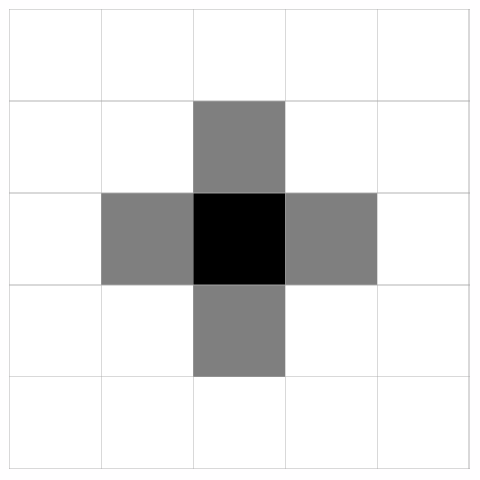
\includegraphics[width=\textwidth]{img/nNeumann.png}
		\caption{Vecindad de Neumann}
		\label{fig:N_neumann}
	\end{subfigure}
	\begin{subfigure}[b]{0.30\textwidth}
		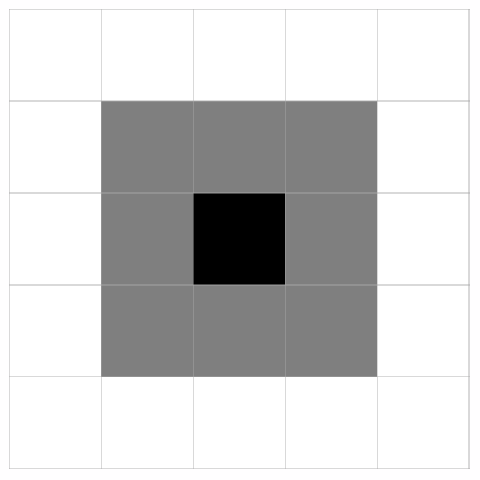
\includegraphics[width=\textwidth]{img/nMoore.png}
		\caption{Vecindad de Moore}
		\label{fig:N_moore}
	\end{subfigure}
	\begin{subfigure}[b]{0.40\textwidth}
		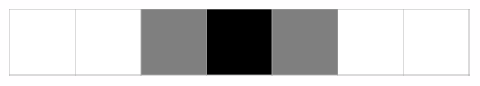
\includegraphics[width=\textwidth]{img/nWolfram.png}
		\caption{Vecindad de radio uno}
		\label{fig:N_wolfram}
	\end{subfigure}
	\caption{Las vecindades \ref{fig:N_neumann} y \ref{fig:N_moore} son para CA bidimensionales; la \ref{fig:N_wolfram} es para CA unidimensionales. La célula negra representa la célula actual y, junto con las grises, conforma su vecindad.}
	
	\label{fig:vecindades_regulares}
	
\end{figure}

Las vecindades no solo son cuadradas; también pueden tener otras formas, como hexágonos o triángulos, que se muestran en las figuras \ref{fig:N_hexagonal} y \ref{fig:N_triangular}.  Además, existen vecindades con comportamiento dinámico, como la vecindad de Margolus mostrada en la figura \ref{fig:N_margolus}, cuya configuración alterna entre dos disposiciones en cada paso evolutivo \cite{margolus}.

\begin{figure}[htbp]
	\centering
	\begin{subfigure}[b]{0.30\textwidth}
		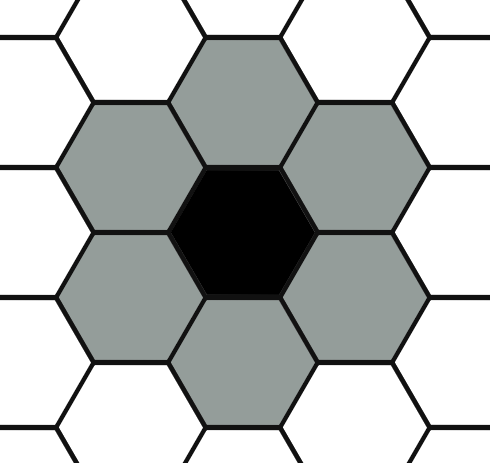
\includegraphics[width=\textwidth]{img/nHexagonal.png}
		\caption{Vecindad hexagonal}
		\label{fig:N_hexagonal}
	\end{subfigure}
	\begin{subfigure}[b]{0.30\textwidth}
		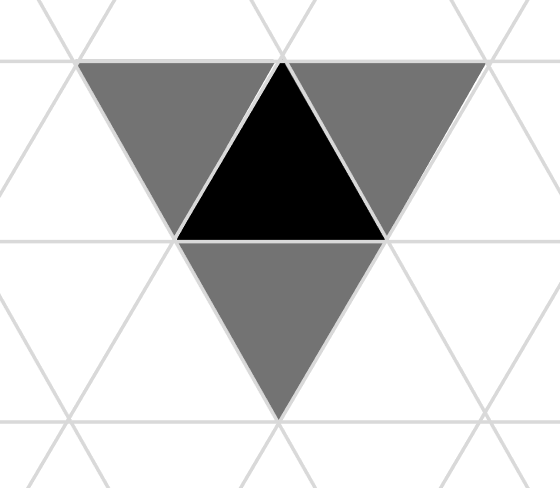
\includegraphics[width=\textwidth]{img/nTriangular.png}
		\caption{Vecindad triangular}
		\label{fig:N_triangular}
	\end{subfigure}
	\begin{subfigure}[b]{0.30\textwidth}
		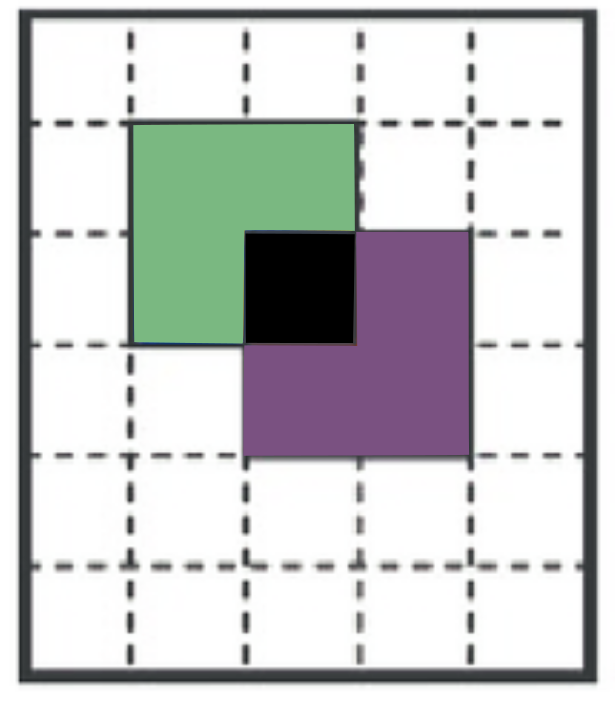
\includegraphics[width=\textwidth]{img/nMargolus.png}
		\caption{Vecindad de Margolus}
		\label{fig:N_margolus}
	\end{subfigure}
	
	\caption{Vecindades para CA bidimensionales. En \ref{fig:N_hexagonal} y \ref{fig:N_triangular}, la célula negra es la actual y las grises conforman su vecindad.  En \ref{fig:N_margolus}, la célula negra es la actual, mientras que las células verdes y moradas representan las vecindades activas en tiempos pares e impares, respectivamente.}
	
	\label{fig:vecindades_irregulares}
	
\end{figure}

\section{Estados}

Cada célula adquiere un único estado $s$ en cada paso de tiempo, donde $s$ pertenece a un conjunto de estados $s \in \mathcal{S}$. Por ejemplo, el autómata celular de John von Neumann contempla 29 estados, aunque algunos autores han propuesto variantes reducidas a cuatro estados, conservando su capacidad de autoreproducirse \cite{ca_phd}. 

Por otro lado, el juego de la vida se compone de dos estados que denominó ``vivas'' y ``muertas'' \cite{life}.  De igual forma, Stephen Wolfram utiliza dos estados en los autómatas celulares elementales \cite{nks}.

Idealmente, el espacio celular $\mathcal{L}$ es infinito, lo que permitiría infinitas combinaciones de estados. Sin embargo, esto es inviable computacionalmente, por lo que, al igual que el autómata celular de John von Neumann, se requiere establecer una restricción de finitud, como lo marca \cite{ca_phd}. 

\begin{definition}
	
	Sea $\mathcal{R}$ la regla local de un autómata celular. Un estado $\sigma_q \in \mathcal{S}$ es inactivo si $\mathcal{R}(\sigma_q, \sigma_q, \dots, \sigma_q) = \sigma_q$.
	
\end{definition}

Es decir, si una célula y todos sus vecinos están en estado inactivo, la célula permanece inactiva tras aplicar $\mathcal{R}$. Cabe notar que todos los vecinos deben estar en dicho estado, por lo que, si alguno cambia, podría reactivarse. 

Para trabajar computacionalmente, \cite{ca_phd} define las configuraciones finitas de la siguiente manera:

\begin{definition}
	
	Sea $\sigma_q \in \mathcal{S}$ un estado inactivo, $\sigma_p \neq \sigma_q \in \mathcal{S}$ un estado no inactivo y sea $\mathcal{L}$ un espacio celular infinito. Se considera que un autómata celular tiene configuración finita si solo un número finito de celdas están en estados activos $\sigma_p$.
	
\end{definition}

Si la configuración inicial es finita, entonces la evolución en el siguiente paso de tiempo también será finita (ver tabla \ref{tab:CA_finito}).

\begin{table}
	
	\centering
	
	\begin{tabular}{c | c c c c c c c c c c c} 
		
		$t$ & \multicolumn{11}{c}{ $\vec{\sigma}(t)$  } \\ \hline \hline
		
		0 & && & \dots & $q$ & $p$ & $q$ & \dots & && \\ \hline
		
		1 & & & \dots & $q$ & $p$ & $p$&  $p$ & $q$ & \dots & & \\ \hline
		
		2  & & \dots & $q$  & $p$ & $p$ & $p$&  $p$ &  $p$& $q$ & \dots &  \\ \hline
		
		3 & \dots & $q$  & $p$ & $p$ & $p$&  $p$&$p$ &$p$& $p$ & $q$ & \dots \\
		
	\end{tabular}
	
	\caption{Evolución temporal de un autómata celular unidimensional con una configuración inicial finita. Donde $p$ representa estados activos y $q$ estados inactivos. Los conjuntos $\vec{\sigma} (t)$ y $\vec{\sigma} (t + 1)$ son finitos.}
	
	\label{tab:CA_finito}
	
\end{table}

Sea $\mathcal{C} =  \mathcal{S}^\mathcal{L}$ el conjunto de todas las configuraciones. Definimos $\mathcal{C}_F \subset \mathcal{C}$ como el subconjunto de todas las configuraciones finitas. Esta restricción es necesaria para hacer computacionalmente viable la simulación de la evolución.

Finalmente, resulta necesario definir un estado estable, el cual servirá más adelante para establecer una clasificación \cite{ca_phd}. 

\begin{definition}
	
	Dado un autómata celular y un estado $s \in \mathcal{S}$, se dice que $s$ es un estado estable si $\mathcal{R}(s, s, \dots, s) = s$.
	
\end{definition}

Esto es, un estado estable $s$ que evoluciona siempre en sí mismo, por lo que $\sigma(t) = \sigma(t + 1)$. 

\section{Condiciones de frontera}

Idealmente, los autómatas celulares pueden evolucionar en espacios infinitos; sin embargo, para su simulación computacional es necesario establecer límites. Estos límites, llamados condiciones de frontera, restringen el espacio celular $\mathcal{L}$ \cite{ca_phd, ca_phd_gua}.

\begin{definition}
	
	Un autómata celular es finito si el espacio celular $\mathcal{L} \subseteq \mathbb{Z}^D$ es finito; en caso contrario, se denomina infinito. 
	
\end{definition}

En un autómata celular finito se consideran principalmente dos tipos de condiciones de frontera: abierta y periódica \cite{ca_phd_gua}.

\begin{itemize}
	
	\item \textbf{Condición de frontera abierta}: Se les asigna un estado fijo a todos aquellos vecinos faltantes en las células de la frontera. 
	
	
	
	\item \textbf{Condición de frontera periódica}: Los vecinos faltantes de las células en la frontera son otras células en la frontera. La figura \ref{fig:B_periodica} muestra cómo se conectan las células de la frontera en un espacio unidimensional.
	
\end{itemize}

\begin{figure}[htbp]
	\centering
	\begin{subfigure}[b]{0.45\textwidth}
		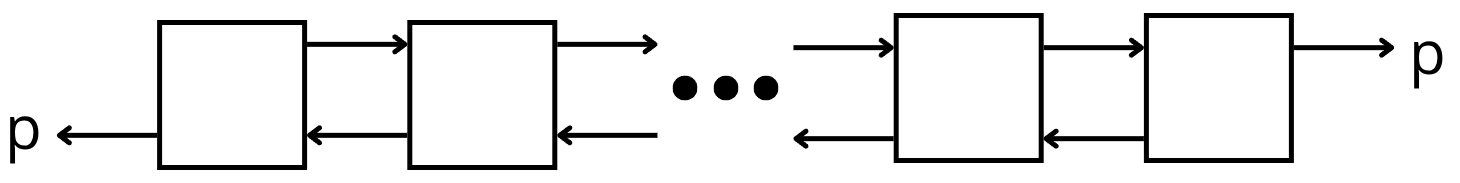
\includegraphics[width=\textwidth]{img/bAbierta.png}
		\caption{Condición de frontera abierta}
		\label{fig:B_abierta}
	\end{subfigure}
	\begin{subfigure}[b]{0.45\textwidth}
		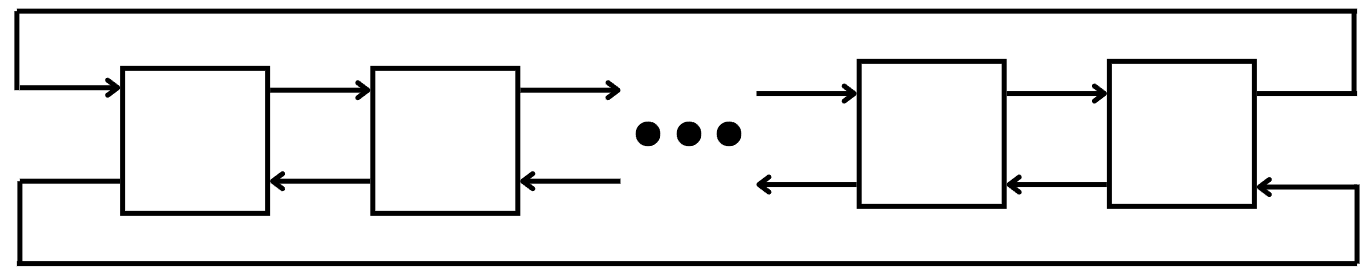
\includegraphics[width=\textwidth]{img/bPeriodica.png}
		\caption{Condición de frontera periódica}
		\label{fig:B_periodica}
	\end{subfigure}
	
	\caption{Condiciones de frontera con dos vecinos. La figura \ref{fig:B_abierta} asigna un estado no inactivo al vecino faltante. La figura \ref{fig:B_periodica} entabla relación de vecindad entre las células en la frontera, formando un anillo.}
	
	\label{fig:fronteras}
	
\end{figure}

Las condiciones de frontera periódica conectan a los autómatas celulares finitos con los infinitos que tienen configuraciones que se repiten \cite{ca_phd}.

\begin{definition}
	
	Una configuración $\vec{\sigma} \in \mathcal{C}$ de un autómata celular $D$-dimensional se dice periódica si es invariante ante un conjunto de traslaciones linealmente independientes en $D$ direcciones. Es decir:
	
	\[
	\vec{\sigma} = T_i^{n_i} (\vec{\sigma}), \; \forall i \in \{ 1,2, \dots, D \}
	\]
	
	donde  $T_i^{n_i}$ denota un desplazamiento de $n_i$ posiciones en la dimensión $i$.
	
\end{definition}

Definimos entonces a $\mathcal{C}_P \subset \mathcal{C}$ como el conjunto de todas las configuraciones periódicas. Estas configuraciones preservan la condición de frontera periódica en cada traslación \cite{ca_phd}. 

La frontera reflectiva asigna a los vecinos faltantes el mismo estado de la célula en la frontera (figura \ref{fig:B_reflectiva}). En este caso, las células de la frontera son vecinas de sí mismas. La frontera reflexiva, en cambio, imita el estado de los vecinos más próximos de la célula en el borde (figura \ref{fig:B_reflexiva}), generando una doble relación de vecindad en los extremos \cite{ca_phd, ca_phd_gua}.

\begin{figure}[htbp]
	\centering
	\begin{subfigure}[b]{0.45\textwidth}
		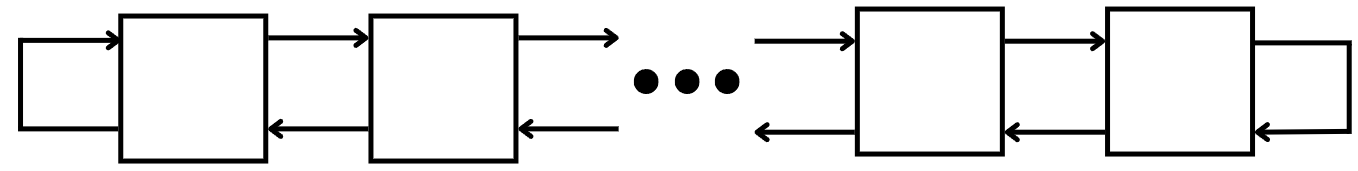
\includegraphics[width=\textwidth]{img/bReflectiva.png}
		\caption{Condición de frontera reflectiva}
		\label{fig:B_reflectiva}
	\end{subfigure}
	\begin{subfigure}[b]{0.45\textwidth}
		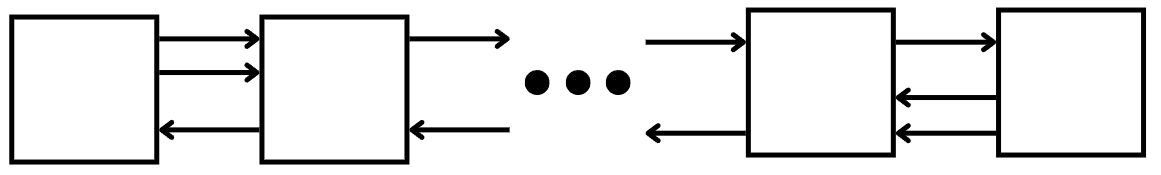
\includegraphics[width=\textwidth]{img/bReflexiva.png}
		\caption{Condición de frontera reflexiva}
		\label{fig:B_reflexiva}
	\end{subfigure}
	
	\caption{Condiciones de frontera con dos vecinos. La figura \ref{fig:B_reflectiva} muestra que las células en la frontera son vecinas entre sí, mientras que la figura \ref{fig:B_reflexiva} indica que las células que están al lado de las células de la frontera pueden tener varios vecinos.}
	
	\label{fig:fronteras_adicionales}
	
\end{figure}

\section{Regla local}

Sea $\mathcal{S}$ el conjunto de estados y $m = |\mathcal{N}|$ el número de vecinos. La función de transición o regla local se define como 

\[
\mathcal{R}: \mathcal{S}^m \to \mathcal{S}
\] 

donde $\mathcal{R}$ asigna un nuevo estado a cada célula en función de los estados de sus $m$ vecinos (incluyéndose a sí misma si aplica).

Para autómatas celulares unidimensionales, dado un rango arbitrario $r$, la regla puede ser escrita como:

\[
\sigma_{i}(t + 1) = \mathcal{R}(\sigma_{i-r}(t), \dots, \sigma_{i}(t), \dots, \sigma_{i+r} (t)), \; \mathcal{R}:  S^{2r + 1} \to S
\]

Donde el rango $r$ especifica el tamaño de la vecindad para cada célula, la cual puede adquirir un valor $k$. Por esto, $\mathcal{R}$ puede ser definido especificando el valor asignado para cada una de las $k^{2r + 1}$ posibles $(2r+1)$-tuplas dada una vecindad.

Un ejemplo de regla local es el juego de la vida \cite{life}. En este caso, el conjunto de estados es binario $\mathcal{S} = \{ 0, 1 \}$, donde $0$ representa células muertas y $1$ las vivas. La regla de transición se define como:

\[
\mathcal{R}: \{ 0, 1 \}^9 \to \{ 0, 1\}
\]

Ya que la vecindad de Moore en 2D involucra 8 vecinos más la propia célula, es decir, $m = 9$. El juego de la vida sigue las siguientes tres reglas:

\begin{itemize}
	
	\item \textbf{Nacimiento}: Una célula muerta en el tiempo $t$ nace en el tiempo $t + 1$ si tiene exactamente tres vecinos vivos en el tiempo $t$.
	
	
	
	\item \textbf{Muerte}: Una célula viva en el tiempo $t$ muere en $t + 1$ por:
	
	\begin{itemize}
		
		\item sobrepoblación; si hay más de tres vecinos vivos en $t$.
		
		\item soledad: si hay menos de tres vecinos vivos en $t$.
		
	\end{itemize}
	
	
	
	\item \textbf{Supervivencia}: Una célula viva en el tiempo $t$ se mantiene viva en $t + 1$ si tiene dos o tres vecinos vivos en $t$.	 
	
\end{itemize}

Se puede usar la notación \textit{Birth/survival} la cual es una dupla de listas que almacenan el número de vecinos vivos que tiene que haber en la vecindad para nacer y para sobrevivir, respectivamente. La configuración para el juego de la vida ``tradicional'' es $B3/S23$, es decir, se requieren 3 células vivas para nacer y se requieren 2 o 3 células vivas para sobrevivir \cite{life}. 

Una regla es semitotalística si la transición depende de la suma de los valores en la vecindad, pero distingue entre diferentes posiciones, como el centro y los bordes. El juego de la vida es un ejemplo de regla semitotalística porque cuenta el número de vecinos vivos, pero trata de forma distinta el estado de la célula central \cite{semi_totalistic}.

En cambio, una regla es totalística si la transición depende únicamente de la suma de los estados en todos los vecinos, sin distinguir posiciones \cite{totalistic}. Por ejemplo, para un autómata celular unidimensional con $|\mathcal{S}| = 3$ estados y radio $r = 1$, solo hay $(|\mathcal{S}|-1) |\mathcal{N}|+1 = (2-1) \cdot 3 + 1 = 4$ posibles valores de suma.

Por otro lado, una regla local arbitraria sí distingue las posiciones de cada elemento en la vecindad. La configuración dada para el autómata celular elemental considera $k = 2$ (es decir, $\sigma_i \in \{0, 1\}$), un radio $r = 1$ ($|\mathcal{N}| = 3$) y la regla $\mathcal{R}: \{0,1\}^3 \rightarrow \{0,1\}$ que se define como:

\[
\phi(\sigma_{i-1}(t), \sigma_{i}(t), \sigma_{i+1}(t))
\]

Esta dinámica está dada por las posibles configuraciones que las tres células adyacentes pueden adquirir en el tiempo $t$. Podemos encontrar $k^{|\mathcal{N}|} = 2^3 = 8$ patrones posibles en la vecindad, número correspondiente a la combinatoria de dos estados en tres posiciones. Cada vez que encontremos un patrón, podemos asignarle un nuevo estado a $\sigma_i(t + 1)$ ($\{ 0, 1 \}$), por lo que el número total de reglas asciende a $k^{k^{|\mathcal{N}|}} = 2^8 = 256$, como se muestra en la tabla \ref{tab:ECA_evolucion}.

\begin{table}
	
	\centering
	
	\begin{tabular}{c c c c c c c c} 
		
		111 & 110 & 101 & 100 & 011 & 010 & 001 & 000 \\
		
		$\downarrow$ & $\downarrow$ & $\downarrow$ & $\downarrow$ & $\downarrow$ & $\downarrow$ & $\downarrow$ & $\downarrow$ \\
		
		$\{ 0, 1 \}$ & $\{ 0, 1 \}$ & $\{ 0, 1 \}$ & $\{ 0, 1 \}$ & $\{ 0, 1 \}$ & $\{ 0, 1 \}$ & $\{ 0, 1 \}$ & $\{ 0, 1 \}$ 
		
	\end{tabular}
	
	\caption{Cada posible combinación de tres células puede adquirir uno de dos valores. Cuando la célula evaluada encaja en este patrón, su valor cambia al establecido por la regla. Este conjunto de 256 forma parte de los autómatas celulares elementales.}
	
	\label{tab:ECA_evolucion}
	
\end{table}

Estas reglas se pueden representar de forma tabular y también como un número decimal. La tabla \ref{tab:ECA_rules} muestra la asociación entre la forma tabular y la regla decimal.

Nótese que la regla decimal solo aplica cuando las condiciones son las mismas. Es decir, cuando el número de vecinos $|\mathcal{N}|$ y estados $|\mathcal{S}|$ son invariantes; a cada regla se le puede asociar un número entero único, pero dos reglas que difieren en vecindad o estados pueden compartir el número decimal. Por ejemplo, considerando la regla $10$ con $|\mathcal{N}| = 2$ y $|\mathcal{S}| = 2$ es $1010$, la cual es completamente diferente cuando $|\mathcal{N}| = 3$ y $|S| = 2$, lo que da como resultado $ 000000101$.

\begin{table}
	
	\centering
	
	\begin{tabular}{c | c c c c c c c c | c} 
		
		\textbf{Binario} &111 & 110 & 101 & 100 & 011 & 010 & 001 & 000 & \multirow{3}{*}{\textbf{regla}} \\ 
		
		\textbf{Decimal} & 7 & 6 & 5 & 4 & 3 & 2 & 1 & 0 & \\ 
		
		\textbf{Valor} & $2^7$ & $2^6$ & $2^5$ & $2^4$ & $2^3$ & $2^2$ & $2^1$ & $2^0$ & \\ \hline
		
		& 0 &  0 &  0 &  0 &  0 &  0 &  0 &  0 & 0 \\
		
		& 0 &  0 &  0 &  0 &  0 &  0 &  0 &  1 & 1 \\
		
		& \multicolumn{8}{c|}{\vdots} & \vdots \\ 
		
		& 0 &  0 &  0 &  1 &  1 &  1 &  1 &  0 & 30 \\
		
		& \multicolumn{8}{c|}{\vdots} & \vdots \\ 
		
		& 0 &  1 &  1 &  0 &  1 &  1 &  1 &  0 & 110 \\
		
		& \multicolumn{8}{c|}{\vdots} & \vdots \\ 
		
		& 1 &  1 &  1 &  1 &  1 &  1 &  1 &  1 & 255 
		
	\end{tabular}
	
	\caption{Los valores binarios representan las posibles configuraciones de estados que pueden aparecer en el espacio, cada uno asociado a un valor decimal, y el valor es la potencia asociada a esa combinación. Para convertir la regla tabular en la decimal, solo es necesario convertir el número binario.} 
	
	\label{tab:ECA_rules}
	
\end{table}

\section{Clasificación}

Stephen Wolfram, al estudiar los autómatas celulares elementales, descubre que existen comportamientos compartidos por ciertas reglas y que dicho comportamiento es inherente a la configuración inicial del espacio celular. Es por esto que define las siguientes clases de comportamiento, ilustradas en la figura \ref{fig:clasificacion}:

\begin{enumerate}[label= \Roman*]
	
	\item Evolucionan a un estado uniforme. 
	
	\item Evolucionan a estados cíclicos aislados.
	
	\item Evolucionan en comportamientos caóticos.
	
	\item Evolucionan en estados complejos aislados.
	
\end{enumerate}

\begin{figure}[htbp]
	\centering
	\begin{subfigure}[b]{0.40\textwidth}
		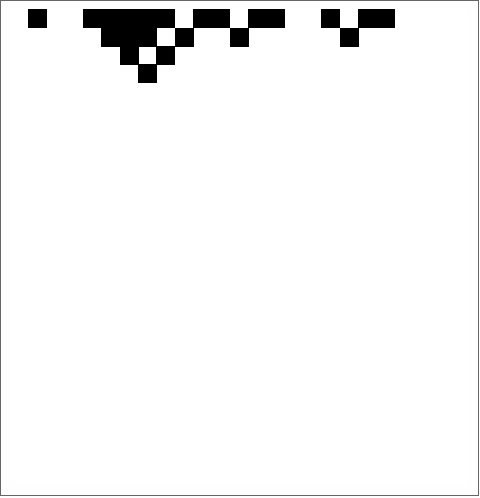
\includegraphics[width=\textwidth]{img/c1.png}
		\caption{Clase I: Regla 160}
		\label{fig:c1}
	\end{subfigure}
	\begin{subfigure}[b]{0.40\textwidth}
		
\includegraphics[width=\textwidth]{img/c2.png}
		\caption{Clase II: Regla 4}
		\label{fig:c2}
	\end{subfigure}
	\begin{subfigure}[b]{0.40\textwidth}
		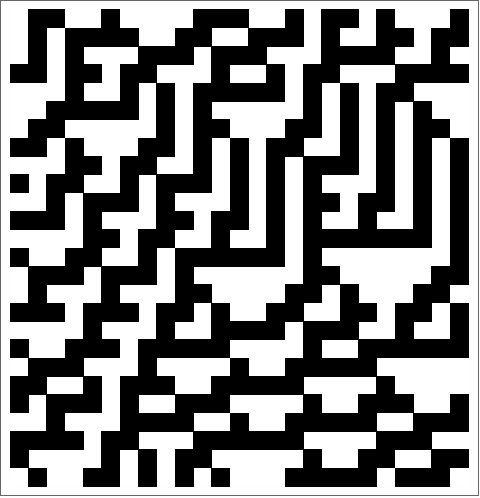
\includegraphics[width=\textwidth]{img/c3.png}
		\caption{Clase III: Regla 30}
		\label{fig:c3}
	\end{subfigure}
	\begin{subfigure}[b]{0.40\textwidth}
		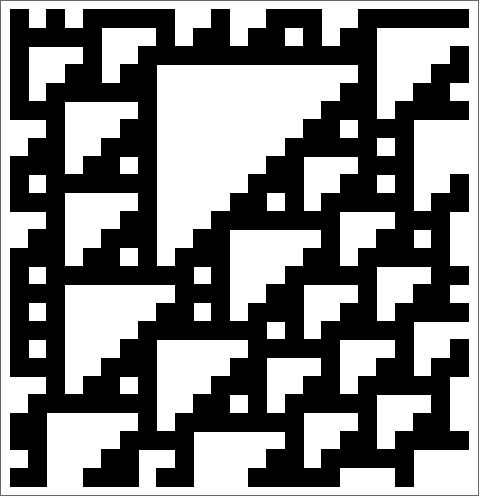
\includegraphics[width=\textwidth]{img/c4.png}
		\caption{Clase IV: Regla 110}
		\label{fig:c4}
	\end{subfigure}
	\caption{Clasificación de Wolfram. Las figuras evolucionan 25 pasos una configuración inicial aleatoria con condición de frontera cíclica.}
	
	\label{fig:clasificacion}
	
\end{figure}

Sin embargo, aunque esta clasificación funciona para los autómatas celulares elementales, existen reglas bajo diferentes configuraciones que pueden pertenecer a múltiples clases o, en el peor de los casos, no pertenecen a ninguna de ellas \cite{gen_Life_campoPromedio}. 

Es por esto que en \cite{CAclassification} proponen una nueva clasificación siguiendo ciertas limitaciones, entre las cuales están:

\begin{itemize}
	
	\item Esta clasificación es para autómatas celulares finitos. 
	
	\item Cada clase es un subconjunto de la siguiente clase.
	
\end{itemize}

\begin{definition}
	
	Un autómata celular es de clase I si existe un estado estable $s \in \mathcal{S}$ tal que todas las configuraciones finitas evolucionan a una configuración homogénea de $s$.
	
\end{definition}

Es decir, dada cualquier configuración inicial en un autómata celular finito, todas las células adquieren el estado $s$ tras cierto número de pasos evolutivos. Esto se aplica a todas las finitas configuraciones iniciales.

\begin{definition}
	
	Un autómata celular es de clase II si existe un estado estable $s \in \mathcal{S}$ tal que se repite a $n$ pasos evolutivos.
	
\end{definition}

Esto implica que la evolución se repite cada $n$ número de pasos ($\sigma(t) = \sigma(t + n)$). Resulta evidente que la clase I está contenida en la clase II, haciendo que $n = 1$, lo que implica un periodo de uno.

Una clasificación es $s$-finita si solo difiere del estado estable en una región finita.

\begin{definition}
	
	Un autómata celular es de clase III si existe un estado estable $s \in \mathcal{S}$ tal que para cualquier par de configuraciones $s$-finitas $C_1$ y $C_2$, es decidible si $C_1$ evoluciona a $C_2$.
	
\end{definition}

Es decir, si podemos determinar en tiempo finito si el CA evoluciona de $C_1$ a $C_2$, entonces pertenece a clase III. En caso contrario, pertenece a la clase IV, la cual contiene a todos los autómatas celulares \cite{CAclassification}.

\begin{definition}
Todos los autómatas celulares pertenecen a la clase IV.	
\end{definition}

Otra clasificación considera extensiones o modificaciones en la definición que alteran el comportamiento del autómata celular. A continuación, se describen algunas de estas extensiones para el modelado de sistemas complejos. 

\begin{itemize}
	
	\item \textbf{Autómatas celulares en grafos}: Amplían la idea de la estructura de red clásica al permitir que las vecindades no sean iguales: cada célula puede tener un número diferente de vecinos. Esta flexibilidad los hace adecuados para modelar fenómenos sobre grafos, como redes sociales o flujos en infraestructura. Sin embargo, diseñar manualmente las reglas de transición en estos entornos es una tarea compleja, lo que ha motivado propuestas como los autómatas celulares neuronales en grafos, que permiten aprender dichas reglas automáticamente \cite{neuripsGCA}.
	
	\item \textbf{Autómatas celulares probabilísticos}: Estos extienden el modelo clásico al incorporar reglas de transición estocásticas. En vez de una evolución que sigue un camino fijo, los estados futuros dependen de probabilidades que se ven afectadas por el entorno. Esto ayuda a entender la incertidumbre, el ruido y los comportamientos que surgen de manera inesperada. Son especialmente útiles para simular dinámicas como propagación de epidemias o sistemas sociales, donde los mecanismos de transición no siempre están completamente definidos \cite{gacsPCA}.
	
	\item \textbf{Autómatas celulares no homogéneos}: Permiten que diferentes células tengan diferentes funciones de transición. Para esto, se utilizan dos planos llamados ``plano de datos'', el cual contiene la evolución del sistema; y ``plano de control'', el cual define las reglas de transición para cada célula. Esto permite estudiar el comportamiento y la interacción entre diferentes reglas que comparten espacio \cite{hartmanIHCA}.
	
	\item \textbf{Autómatas celulares continuos}: Son autómatas celulares que pueden ser continuos en los estados, en el tiempo y en el espacio \cite{nks}:
	
	\begin{itemize}
		\item Los estados continuos adquieren valores reales y no solo enteros.
		
		\item El tiempo continuo se define mediante una función que determina el intervalo de espera para actualizar la célula en función de su estado actual.
		
		\item El espacio continuo se obtiene al asignar diferentes pesos a las células dentro de la vecindad \cite{beckerCCA}.
	\end{itemize}
\end{itemize}

Aunque estas variantes han ampliado el uso de los autómatas celulares, un problema que se repite es definir correctamente las reglas de transición para lograr un fenómeno específico. Este desafío ha llevado a la creación de autómatas celulares neuronales. En estos, la función de transición no se define de manera clara, sino que se aprende a través de una red neuronal artificial. Pero antes de definirlos, es necesario comprender qué son las redes neuronales.

\clearpage